\section{Theory}
\subsection{Spontaneous parametric down-conversion }
To exploit the advantages of quantum imaging and sensing, one needs to create correlated biphoton states of light. One approach to create such quantum states are sources using \acrfull{spdc}. 
The underlying process is as follows: an incident pump photon with frequency $\omega_{\text{p}}$ causes a nonlinear material response resulting in the spontaneous emission of a photon pair with lower frequencies $\omega_{\text{s}}$ and $\omega_{\text{i}}$. The subscripts $s$ and $i$ represent the signal and idler photons, as they are usually referred to. \newline
To achieve efficient \acrshort{spdc} processes, the energy and momentum must be conserved. This means that the photon pair must interfere constructively and fulfill the phase-matching conditions \cite{gilabertebassetPerspectivesApplicationsQuantum2019} : 
\begin{equation}
	\begin{aligned}
		\omega_{\text{p}} &= \omega_{\text{s}} + \omega_{\text{i}} \\
		\myvect{k}_{\text{p}} &= \myvect{k}_{\text{s}} + \myvect{k}_{\text{i}} - \Delta \myvect{k}
	\end{aligned}
\end{equation}
where the indices p, s and i refer to the pump, signal and idler photon. $\Delta k$ represents the phase mismatch caused by dispersion, which limits the efficiency of the photon pair generation. A visualization of the conservation processes is shown in \autoref{fig:SPDC}. \newline
Most experiments use crystals, such as \acrfull{ktp} and \acrfull{bbo}, or waveguides like \acrfull{ln}, because they exhibit second-order nonlinearity \cite{fiorentinoSpontaneousParametricDownconversion2007,kwiatUltrabrightSourcePolarizationentangled1999,tanzilliHighlyEfficientPhotonpair2000}.\newline
There are two approaches to compensate for the mismatch.
One is called \acrfull{qpm} and can be achieved in periodically poled crystals, e.g. \acrshort{ktp} or \acrshort{ln}, where the nonlinear response also changes periodically, which compensates the mismatch. It allows for a process called type-0 \acrshort{spdc} to happen, which means that all three photons (pump, signal, idler) have the same polarization. \newline
Another way to compensate the mismatch is called \acrfull{bpm} and uses anisotropic materials, such as \acrshort{bbo}, as the refractive index changes with the polarization of the incident photon. The effect of using \acrshort{bpm} is that the extraordinary photon is always polarized perpendicular to the pump. Therefore, no type-0 \acrshort{spdc} can be achieved with this approach. The two other possible cases are called type-I and type-II \acrshort{spdc}. In type-I \acrshort{spdc} the signal and idler photons share the same polarization and are polarized perpendicular to the pump, while in type-II \acrshort{spdc} the signal and idler photons are polarized perpendicular to each other \cite{boydNonlinearOptics2008}. \newline
\begin{figure}[!bt]
	\centering
	\resizebox{.65\textwidth}{!}{%
		\begin{tikzpicture}
			\tikzstyle{every node}=[font=\LARGE]
			
			\pgfmathsetmacro{\yTop}{12.5}
			\pgfmathsetmacro{\yBottom}{9.25}
			\pgfmathsetmacro{\yMid}{\yBottom + 0.6*(\yTop - \yBottom)}
			\pgfmathsetmacro{\pLab}{\yBottom + 0.5*(\yTop - \yBottom)}
			\pgfmathsetmacro{\sLab}{\yBottom + 0.3*(\yTop - \yBottom)}
			\pgfmathsetmacro{\iLab}{\yBottom + 0.8*(\yTop - \yBottom)}
			
			
			\draw [line width=2.5pt] (3.5,\yBottom) -- (12.5,\yBottom);
			\draw [ color={rgb,255:red,0; green,0; blue,255}, line width=2pt,-{Latex[length=4mm]}] (5,\yBottom) -- (5,\yTop);
			\draw [line width=2.3pt, dashed] (3.75,\yTop) -- (12.5,\yTop);
			\draw [ color={rgb,255:red,255; green,0; blue,0}, line width=2pt,-{Latex[length=4mm]}] (10,\yTop) -- (10,\yMid);
			\draw [ color=black!40!green, line width=2pt,-{Latex[length=4mm]}] (10,\yMid) -- (10,\yBottom);
			\node [font=\LARGE, color={rgb,255:red,0; green,0; blue,255}] at (4.25,\pLab) {$\omega_{\text{p}}$};
			\node [font=\LARGE, color={rgb,255:red,255; green,0; blue,0}] at (10.5,\iLab) {$\omega_{\text{i}}$};
			\node [font=\LARGE, color=black!40!green] at (10.5,\sLab) {$\omega_{\text{s}}$};
			\draw [ color={rgb,255:red,0; green,0; blue,255}, line width=2pt, -{Latex[length=4mm]}] (15,10.25) -- (20.25,10.25);
			\draw [ color={rgb,255:red,0; green,0; blue,0}, line width=2pt, -{Latex[length=4mm]}] (20.25,10.25) -- (21.25,10.25);
			\draw [ color={rgb,255:red,255; green,0; blue,0}, line width=2pt, -{Latex[length=4mm]}] (15,11.5) -- (17.5,11.5);
			\draw [ color=black!40!green, line width=2pt, -{Latex[length=4mm]}] (17.5,11.5) -- (21.25,11.5);
			
			\node [font=\LARGE, color={rgb,255:red,0; green,0; blue,255}] at (17.5,9.5) {$k_{\text{p}}$};
			\node [font=\LARGE, color={rgb,255:red,0; green,0; blue,0}] at (20.75,9.5) {$\Delta k$};
			\node [font=\LARGE, color={rgb,255:red,255; green,0; blue,0}] at (16.25,12) {$k_{\text{i}}$};
			\node [font=\LARGE, color=black!40!green] at (19.5,12) {$k_{\text{s}}$};
			
			\node [font=\LARGE] at (8,13.75) {$Energy\,\,conservation$};
			\node [font=\LARGE] at (18,13.75) {$Momentum\,\,conservation$};
			
			% Coordinates
			\coordinate (A) at (7,6.5);
			\coordinate (B) at (10.5,6.5);
			%
			\coordinate (B') at (14.5,7);
			\coordinate (B'') at (14.5,6);
			\coordinate (C') at (18,7);
			\coordinate (C'') at (18,6);
			
			%Rectangle
			%\draw[thick, fill=black!10] (10.5,5.8) rectangle (14.5,7.2);	
			%\node at (12.6,6.5) {$\chi^2$};
			% Rays
			%\draw[line width=2.5pt, rayE2,color=blue] (A) -- (B);
			
			%% Bottom Ray
			%\draw[line width=2.5pt, rayE2,color=black!40!green] (B') -- (C');
			%\draw[line width=2.5pt, rayE2,color=red] (B'') -- (C'');
			
			% Nodes
			%\node at (1.2,2.4) [color=blue] {\small $\lambda_{\text{p}}$};
			%\node at (6.8,2.9) [color=green] {\small $\lambda_{\text{i}}$};
			%\node at (6.8,0.4) [color=red] {\small $\lambda_{\text{s}}$};
			
		\end{tikzpicture}
	}%
	
	\caption{Conservation processes of collinear Type-0 SPDC}
	\label{fig:SPDC}
\end{figure} 
In this work, the temporal correlation between the signal and idler photons is most commonly used for coincidence measurements. A tool for visualizing the coincidences is a coincidence histogram. These histograms show the number of coincident events as a function of the delay between the arrival times of the photons at two single-photon detectors. \newline
Ideally, the temporal correlation of the photon pairs results in a distinct coincidence peak centered at zero delay if both detectors are the same distance from the \acrshort{spdc} source. 
The width of this peak depends on several factors, including the resolution of the time-tagging electronics that create a timestamp for each detection event and also on the properties of the generated photon pair. \newline
These correlations are evaluated by defining a temporal interval around the detection peak. Within this interval, detection events are considered true coincidences, meaning they originate from the same source. This interval is usually referred to as the coincidence window $\tau_{\text{cw}}$. Events that fall outside this window are usually attributed to uncorrelated background noise and are called accidental counts. A representative scheme of a coincidence histogram is shown in \autoref{fig:HistoExample} .
\begin{figure}[h!]
	\centering
	\resizebox{.6\textwidth}{!}{%
	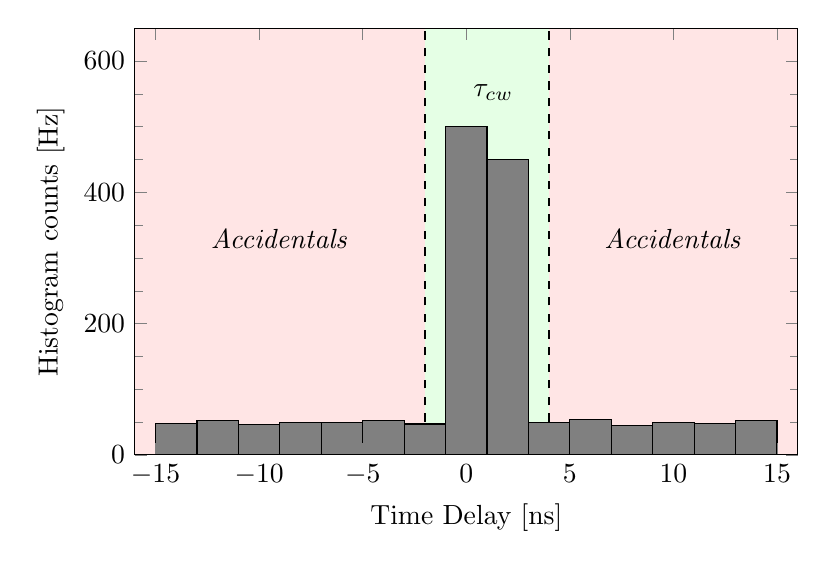
\begin{tikzpicture}
		\begin{axis}[
			ymin=0,
			ymax=650,
			xmin=-16,
			xmax=16,
			xlabel={Time Delay [ns]},
			ylabel={Histogram counts [Hz]},
			xtick={-15,-10,-5,0,5,10,15},
			bar width=2,
			minor y tick num = 3,
			area style,
			width=10cm,
			height=7cm,
			every axis plot/.append style={fill=gray!40}
			]
			
			% Shaded left region: x < -5
			\addplot [
			red,
			fill=red,
			fill opacity=0.1,
			draw=none
			] coordinates {
				(-16,650)
				(-2,650)
				(-2,0)
				(-16,0)
			};

			\addplot [
			red,
			fill=green,
			fill opacity=0.1,
			draw=none
			] coordinates {
				(-2,650)
				(4,650)
				(4,0)
				(-2,0)
			};
			
						
			% Shaded right region: x > 5
			\addplot [
			red,
			fill=red,
			fill opacity=0.1,
			draw=none
			] coordinates {
				(4,650)
				(16,650)
				(16,0)
				(4,0)
			};
			
			% Vertical dashed line at x = -5
			\draw[dashed, thick] (axis cs:-2,0) -- (axis cs:-2,650);
			
			% Vertical dashed line at x = 5
			\draw[dashed, thick] (axis cs:4,0) -- (axis cs:4,650);
			
			\node at (axis cs:-9, 300) [anchor=south] {\textit{Accidentals}};
			
			\node at (axis cs:10, 300) [anchor=south] {\textit{Accidentals}};
			
			\node at (axis cs:1.3, 525) [anchor=south] {$\tau_{\text{cw}}$};
									
			\addplot+ [ybar interval,mark=no] plot coordinates {
				(-15, 48)
				(-13, 52)
				(-11, 46)
				(-9, 50)
				(-7, 49)
				(-5, 53)
				(-3, 47)
				(-1, 500)
				(1, 450)
				(3, 49)
				(5, 54)
				(7, 45)
				(9, 50)
				(11, 48)
				(13, 52)
				(15, 49)
			};
			
		\end{axis}
	\end{tikzpicture}
	}%
	\caption{Schematic of a coincidence histogram}
	\label{fig:HistoExample}
\end{figure} 
%\todo[inline]{histogram, correlations, how that works}
%\newpage
\subsection{Model for transmittance estimation}
%\vspace{-0.5em}
When noise is present in the experimental setup, the question arises as to how precisely the parameters of interest can be determined using either the conventional or coincidence approach. As the objective of this work is to compare both methods in terms of the precision of the measurement rather than focusing on the estimated absolute values, it is the variance of the chosen parameter that is decisive. Since the results of this study will be applied in a transmission setup, the transmittance of the sample is chosen as the key parameter. \newline
In the following, the formulas to calculate the variance of the transmittance are derived both for the conventional and coincidence approach. The arm in which the sample is placed will be referred to as idler and the other arm, the reference arm, as signal. The case in which a sample is placed in the idler arm is denoted with the superscript '$\text{sam}$', where there is no sample with '$\text{ref}$'. \newline
Starting with the conventional approach, only the idler arm is required. Therefore, in absence of the sample, the number of total detected counts in this arm is: 
\begin{equation}
	N_{\text{tot}}^{\text{ref}} = \eta_{\text{idl}} \, N_g + N_{\text{noise}}^{\text{ref}}
	\label{eq:SingleRef}
\end{equation}
where $N_{\text{tot}}^{\text{ref}}$ is the total number of counts without a sample, $\eta_{\text{idl}}$ is the efficiency of the idler arm, $N_g$ is the number of generated photon pairs and $N_{\text{noise}}^{\text{ref}}$ is the number of counts when there are no photon pairs, which refer to noise consisting of e.g. dark counts of the detector or stray light. \newline
When a sample is placed in the idler arm, the total number of counts changes according to the transmittance of the material. Therefore, \autoref{eq:SingleRef} is modified as follows:
\begin{equation}
	N_{\text{tot}}^{\text{sam}} = T \, \eta_{\text{idl}} \, N_g + N_{\text{noise}}^{\text{sam}}
	\label{eq:SingleSam}
\end{equation}
where $N_{\text{tot}}^{\text{sam}}$ represents the total counts in presence of a sample and $T$ is the transmittance of the sample. \newline
$T$ can be calculated combining equations \ref{eq:SingleRef} and \ref{eq:SingleSam}:
\begin{equation}
	T = 
	\frac{\,N_{\text{tot}}^{\text{sam}} - N_{\text{noise}}^{\text{sam}}\,}
	{\,N_{\text{tot}}^{\text{ref}} - N_{\text{noise}}^{\text{ref}}\,}
	\label{eq:TransSingle}
\end{equation}
As can be seen from the formula, four independent measurements must be conducted to retrieve the transmittance: two where only the dark counts are measured with and without the sample, and two with an active laser also with and without the sample. 
\newpage
Based on \autoref{eq:TransSingle} and error propagation, the variance of the transmittance $\operatorname{Var}(T)$ can be calculated assuming that all four variables are independent of each other \cite{kuNotesUsePropagation1966}: 
\begin{equation}
	\begin{aligned}
		\operatorname{Var}(T) 
		&= \sum_{i} \left( \frac{\partial T}{\partial X_i} \right)^{2} 
		\operatorname{Var}\!\left( X_i \right) \\[0.75em]
		&= \left( \frac{\partial T}{\partial N_{\text{tot}}^{\text{sam}}} \right)^{2} 
		\operatorname{Var}\!\left( N_{\text{tot}}^{\text{sam}} \right)
		+ \left( \frac{\partial T}{\partial N_{\text{noise}}^{\text{sam}}} \right)^{2} 
		\operatorname{Var}\!\left( N_{\text{noise}}^{\text{sam}} \right) \\[0.75em]
		&\quad + \left( \frac{\partial T}{\partial N_{\text{tot}}^{\text{ref}}} \right)^{2} 
		\operatorname{Var}\!\left( N_{\text{tot}}^{\text{ref}} \right)
		+ \left( \frac{\partial T}{\partial N_{\text{noise}}^{\text{ref}}} \right)^{2} 
		\operatorname{Var}\!\left( N_{\text{noise}}^{\text{ref}} \right)
	\end{aligned}
	\label{eq:VarianceTransGen}
\end{equation}
When the partial derivatives are explicitly calculated using \autoref{eq:TransSingle} the final formula for the variance of the transmittance is:
\begin{equation}
		\operatorname{Var}(T) 
		= \left( \frac{1}{\eta_{\text{idl}}\,N_g} \right)^{2}
		\Bigg[
		\operatorname{Var}\!\left(N_{\text{tot}}^{\text{sam}}\right) 
		+ \operatorname{Var}\!\left(N_{\text{noise}}^{\text{sam}}\right) 
		+ T^{2} \Big[ 
		\operatorname{Var}\!\left(N_{\text{tot}}^{\text{ref}}\right) 
		+ \operatorname{Var}\!\left(N_{\text{noise}}^{\text{ref}}\right) 
		\Big]
		\Bigg]
	\label{eq:VarianceTransExpl}
\end{equation}
\begin{comment}
	\begin{equation}
		\begin{aligned}
			\operatorname{Var}(T) 
			= \left( \frac{1}{\eta_{\text{idl}}\,N_g} \right)^{2}
			\Bigg[
			\operatorname{Var}\!\left(N_{\text{tot}}^{\text{sam}}\right) 
			+ \operatorname{Var}\!\left(N_{\text{noise}}^{\text{sam}}\right) 
			+ T^{2} \Big( 
			\operatorname{Var}\!\left(N_{\text{tot}}^{\text{ref}}\right) 
			+ \operatorname{Var}\!\left(N_{\text{noise}}^{\text{ref}}\right) 
			\Big)
			\Bigg]
			\operatorname{Var}(T) 
			&= \frac{1}{\big( N_{\text{tot}}^{\text{ref}} - N_{\text{noise}}^{\text{ref}} \big)^{2}}
			\Big[ \operatorname{Var}\!\left( N_{\text{tot}}^{\text{sam}} \right)
			+ \operatorname{Var}\!\left( N_{\text{noise}}^{\text{sam}} \right) \Big] \\[0.75em]
			&\quad + \frac{\big( N_{\text{tot}}^{\text{sam}} - N_{\text{noise}}^{\text{sam}} \big)^{2}}
			{\big( N_{\text{tot}}^{\text{ref}} - N_{\text{noise}}^{\text{ref}} \big)^{4}}
			\Big[ \operatorname{Var}\!\left( N_{\text{tot}}^{\text{ref}} \right)
			+ \operatorname{Var}\!\left( N_{\text{noise}}^{\text{ref}} \right) \Big]
		\end{aligned}
		\label{eq:VarianceTransExpl}
	\end{equation}
\end{comment}
When using the coincidence approach, the formulas for the transmittance and it's variance differ. In addition to the idler arm, the signal arm is required to detect correlated photons created by \acrshort{spdc}. Assuming perfectly correlated photon pairs, the formula for pure coincidence counts with and without a sample in the idler arm is as follows \cite{hayatTheoryPhotonCoincidence1999}:
\begin{equation}
	\begin{aligned}
		N_{\text{cc}}^{\text{pure,sam}} &= T \,\eta_{\text{idl}} \,\eta_{\text{sig}} \, N_g, \\[0.5em]
		N_{\text{cc}}^{\text{pure,ref}} &= \eta_{\text{idl}} \,\eta_{\text{sig}} \, N_g
	\end{aligned}
	\label{eq:pureCoinc}
\end{equation}
where $\eta_{\text{sig/idl}}$ is the efficiency of signal and idler arm, $T$ is the transmittance of the sample and $N_g$ is the number of generated photon pairs. \newline
In the context of coincidence measurements, it is important to note that the detection of pure coincidences is not the only outcome of such measurements. In addition to these, what is called accidental counts are also detected. Consequently, instead of both photons originating from one pair being detected simultaneously, only one is detected in one arm and a noise photon is detected in the other.Another possibility is that two photons are detected concurrently in both arms, yet neither of them originates from a \acrshort{spdc}-pair. In both cases, the time tagging unit recognizes them as coincidence events. Hence, they are designated as accidental counts. \newline
The following formula is used to model the accidental counts with sample $\left(R_{\text{ac}}^{\text{sam}} \right)$ and without $\left(R_{\text{ac}}^{\text{ref}} \right)$ \cite{hayatTheoryPhotonCoincidence1999}:
\begin{equation}
	\begin{aligned}
		R_{\text{ac}}^{\text{sam}} 
		&= \Big( T\,\eta_{\text{idl}} R_g + R_{\text{dc,idl}} - R_{\text{cc}}^{\text{pure,sam}} \Big) \,
		\Big( \eta_{\text{sig}} R_g + R_{\text{dc,sig}} - R_{\text{cc}}^{\text{pure,sam}} \Big) \,
		\tau_{\text{cw}} \\[0.75em]
		R_{\text{ac}}^{\text{ref}} 
		&= \Big( \eta_{\text{idl}} R_g + R_{\text{dc,idl}} - R_{\text{cc}}^{\text{pure,ref}} \Big) \,
		\Big( \eta_{\text{sig}} R_g + R_{\text{dc,sig}} - R_{\text{cc}}^{\text{pure,ref}} \Big) \,
		\tau_{\text{cw}}
	\end{aligned}
	\label{eq:AccCounts}
\end{equation}
where the variable $R$ denotes the rate of the respective parameters. The total number can be calculated by multiplying the rate by the exposure time. When the exposure time is set to one second, the rate and the total number coincide. $R_{\text{dc,idl/sig}}$ denotes the dark count rate in the idler/signal arm and $\tau_{cw}$ is the coincidence window.\newline
Therefore, the measured total coincidence events are the sum of pure and accidental coincidence events:
\begin{equation}
	\begin{aligned}
		N_{\text{tot,cc}}^{\text{sam}} &= N_{\text{cc}}^{\text{pure,sam}} + N_{\text{ac}}^{\text{sam}}, \\[0.5em]
		N_{\text{tot,cc}}^{\text{ref}} &= N_{\text{cc}}^{\text{pure,ref}} + N_{\text{ac}}^{\text{ref}}
	\end{aligned}
	\label{eq:totCoinc}
\end{equation}
Using equations \ref{eq:pureCoinc}, \ref{eq:AccCounts} and \ref{eq:totCoinc}, the transmittance $T$ in the coincidence approach can be obtained as follows:
\begin{equation}
	T = 
	\frac{\,N_{\text{tot,cc}}^{\text{sam}} - N_{\text{ac}}^{\text{sam}}\,}
	{\,N_{\text{tot,cc}}^{\text{ref}} - N_{\text{ac}}^{\text{ref}}\,}
	\label{eq:TransCoinc}
\end{equation}
In comparison to the conventional approach from \autoref{eq:TransSingle}, which necessitates four independent measurements, this approach requires only two: one with and one without the sample. This is due to the fact that  accidentals and coincidences can be obtained within a single measurement. \newline
Since the objective is to compare the precision of the transmittance $T$ using the two different approaches, analogue to \autoref{eq:VarianceTransGen}, variance of the transmittance can be calculated using error propagation and coincidence counts:
\begin{equation}
	\begin{aligned}
		\operatorname{Var}(T) 
		&= \sum_{i} \left( \frac{\partial T}{\partial X_i} \right)^{2} 
		\operatorname{Var}\!\left(X_i\right) \\[0.5em]
		&= \left( \frac{\partial T}{\partial N_{\text{tot,cc}}^{\text{sam}}} \right)^{2} 
		\operatorname{Var}\!\left(N_{\text{tot,cc}}^{\text{sam}}\right)
		+ \left( \frac{\partial T}{\partial N_{\text{ac}}^{\text{sam}}} \right)^{2} 
		\operatorname{Var}\!\left(N_{\text{ac}}^{\text{sam}}\right) \\[0.5em]
		&\quad + \left( \frac{\partial T}{\partial N_{\text{tot,cc}}^{\text{ref}}} \right)^{2} 
		\operatorname{Var}\!\left(N_{\text{tot,cc}}^{\text{ref}}\right)
		+ \left( \frac{\partial T}{\partial N_{\text{ac}}^{\text{ref}}} \right)^{2} 
		\operatorname{Var}\!\left(N_{\text{ac}}^{\text{ref}}\right)
	\end{aligned}
	\label{eq:VarianceTransGenCoinc}
\end{equation}
Using equations \ref{eq:pureCoinc} and \ref{eq:totCoinc}, an explicit expression for variance of the transmittance can be obtained:
 \begin{equation}
 	\operatorname{Var}(T) 
 	= \left( \frac{1}{\eta_{\text{sig}}\,\eta_{\text{idl}}\,N_g} \right)^{2}
 	\Bigg[
 	\operatorname{Var}\!\left(N_{\text{tot,cc}}^{\text{sam}}\right) 
 	+ \operatorname{Var}\!\left(N_{\text{ac}}^{\text{sam}}\right) 
 	+ T^{2} \Big[ 
 	\operatorname{Var}\!\left(N_{\text{tot,cc}}^{\text{ref}}\right) 
 	+ \operatorname{Var}\!\left(N_{\text{ac}}^{\text{ref}}\right) 
 	\Big]
 	\Bigg]
 	\label{eq:VarianceTransExplCoinc}
 \end{equation}
 
The objective of this work is to ascertain parameter configurations in which the coincidence approach exhibits superiority in terms of precision, as measured by the magnitude of variance of the transmittance, in comparison to the conventional approach. In order to model both variance formulas properly, it is necessary to experimentally investigate the statistics of each parameter of which the variance is calculated.
\subsection{Photon statistics}
When investigating the statistical properties of photons, it is essential to recognize that different types of light sources exhibit distinct statistical distributions. These distributions are typically characterized by their respective variances, which serve as key indicators of the underlying photon statistics. A coherent laser source is often used as the reference standard, as it represents the most stable form of light emission within the picture of classical optics \cite{foxQuantumOpticsIntroduction2006}. In the following, two types of light sources with fundamentally different statistical distributions are examined in greater detail, namely coherent and thermal sources.

\subsubsection{Coherent light}\label{sec:cohLight}
From a classical perspective, a coherent light field, such as that produced by a stable laser, may be regarded as a monochromatic electromagnetic wave with well-defined amplitude and phase. \newline
When considering a light beam of constant power $P$, the photon flux is uniform in time. To describe the detection statistics, the observation time interval $T$ may be subdivided into a large number of subintervals of duration $\Delta t$. For each subinterval, the probability of detecting a single photon is small but finite. The probability of detecting two or more photons within a single subinterval can be neglected. \newline
Since the intensity of the beam is constant, the detection probability is identical for each subinterval, and successive detection events are statistically independent.  \newline
The probability of detecting $n$ photons within $N$ subintervals of the total observation time $T$ corresponds to the case where $n$ subintervals each contain exactly one photon, while the remaining $(N-n)$ subintervals contain none. This situation is described by the binomial distribution~\cite{foxQuantumOpticsIntroduction2006}:
\begin{equation}
	\mathcal{P}(n) = \frac{N!}{n!\,(N-n)!}\,p^{n}(1-p)^{N-n}
	\label{eq:BinomCoherent}
\end{equation}
where $p$ denotes the probability of detecting a photon in a single subinterval. This probability is equal to the average number of detected photons $\langle n\rangle$ in the observation interval divided by the number of subintervals $N$:
\begin{equation}
	p = \frac{\langle n\rangle}{N}
\end{equation}
Substituting this expression into \autoref{eq:BinomCoherent} yields:
\begin{equation}
	\mathcal{P}(n) = \frac{N!}{n!\,(N-n)!}\,
	\left(\frac{\langle n\rangle}{N}\right)^{n}
	\left(1-\frac{\langle n\rangle}{N}\right)^{N-n}
\end{equation}
In the limit $N \to \infty$, it can be shown~\cite{foxQuantumOpticsIntroduction2006} that the probability of detecting $n$ photons in a coherent light beam reduces to:
\begin{equation}
	\mathcal{P}(n) = \frac{\langle n\rangle^{\,n}}{n!}\,e^{-\langle n\rangle}
\end{equation}
This result corresponds to a \textbf{Poisson distribution}, which is characteristic for coherent light sources. A distinctive property of the Poisson distribution is that the mean photon number $\langle n \rangle$ is equal to its variance, i.e. $\langle n \rangle = \operatorname{Var}(n)$. \newline
Furthermore, it has been demonstrated that the coincidence counts of photon pairs generated via \acrshort{spdc} also follow a Poissonian distribution, since the \acrshort{spdc} process preserves the coherence of the incident pump laser~\cite{avenhausPhotonNumberStatistics2008,schneelochIntroductionAbsoluteBrightness2019,kimPhotoncountingStatisticsbasedSupport2022}. Consequently, the variance of the coincidence counts in \autoref{eq:VarianceTransExplCoinc} can likewise be approximated by their mean value, $ \operatorname{Var}(N_{\text{tot,cc}}) \approx \langle N_{\text{tot,cc}} \rangle$.

\subsubsection{Thermal light}
In contrast to coherent light sources, which exhibit Poissonian photon statistics, thermal light displays fundamentally different statistical properties. Thermal radiation arises from the random emission of photons in a hot body, where the optical field consists of a large number of independently oscillating modes. Each mode can occupy quantized energy levels depending on their angular frequency $\omega$: 
\begin{equation}
	E_n = \left(n + \tfrac{1}{2}\right)\hbar \omega, 
	\qquad n \geq 0,
\end{equation}
where $n$ denotes the photon number. \newline
Using the quantization of energy levels and Planck's law,
the probability of finding $n$ photons in a single mode is then governed by Boltzmann’s law:
\begin{equation}
	\mathcal{P}_{\omega}(n) = \frac{\exp\!\left(-n\hbar\omega / k_B T\right)}
	{\sum_{m=0}^{\infty} \exp\!\left(-m\hbar\omega / k_B T\right)}
	\label{eq:BoltzLaw}
\end{equation}
It can be shown that the mean photon number $\langle n\rangle$ can be expressed as:
\begin{equation}
	\langle n\rangle = \frac{1}{\exp\!\left(\hbar\omega / k_B T\right) -1}
\end{equation}
Substituting this expression into \autoref{eq:BoltzLaw}, the probability distribution can be rewritten as follows:
\begin{equation}
	\mathcal{P}_{\omega}(n) = \frac{1}{\langle n\rangle+1}\left(\frac{\langle n\rangle}{\langle n\rangle+1}\right)^n
	\label{eq:smBE}
\end{equation}
This distribution is referred to as single-mode \textbf{Bose-Einstein distribution} \cite{foxQuantumOpticsIntroduction2006}. \newline
In practice, thermal light sources generally populate a large number of independent modes. Consequently, the multi-mode expansion of the Bose-Einstein distribution must be considered. Assuming that $m$ modes of the field are occupied and that the thermal light is fully unpolarized, the \acrfull{mmbe} distribution can be expressed as~\cite{mandelOpticalCoherenceQuantum1995}:
\begin{equation}
	\mathcal{P}_m(n) = \frac{(n+m-1)!}{(m-1)!\,n!}\,
	\frac{\langle n\rangle^{\,n}}{\left(1+\langle n\rangle/m\right)^{m}\,\left(\langle n\rangle+m\right)^{n}} 
	\label{eq:mmBE}
\end{equation}
The combinatorial prefactor accounts for the number of ways in which $n$ photons can be distributed among $m$ modes, while the remaining factor describes the joint probability associated with the $m$ occupied modes. As a consistency check, it is readily verified that for $m=1$ the expression reduces to the single-mode Bose-Einstein distribution given in \autoref{eq:smBE}.  \newline
The variance of the photon number in the \acrshort{mmbe} distribution is given by:
\begin{equation}
	\operatorname{Var}(n) = \langle n\rangle\left(1+\frac{\langle n\rangle}{m}\right)
	\label{eq:VariancemmBE}
\end{equation}
When compared to the variance of a Poissonian distribution, which is equal to its mean value, it is evident that the \acrshort{mmbe} distribution always exhibits larger fluctuations. Hence, thermal light is intrinsically super-Poissonian. This property is commonly described in terms of photon bunching, meaning that photons tend to arrive in groups more frequently than would be expected for the random distribution characteristic of coherent (Poissonian) light. \newline
From this perspective, coherent sources represent the most stable classical form of light in terms of intensity, while any source with time-dependent fluctuations, such as thermal radiation, necessarily shows enhanced photon-number fluctuations and thus super-Poissonian statistics. \newline
In the limit $m \to \infty$, the variance of the \acrshort{mmbe} distribution approaches the Poissonian result, as can be seen directly from \autoref{eq:VariancemmBE}. This reflects the fact that in the presence of infinitely many modes, the photon statistics become indistinguishable from those of a coherent source. \newline
It was shown that each photon from a \acrshort{spdc} process exhibits \acrshort{mmbe} statistics, whether it is a signal or idler photon \cite{kimPhotoncountingStatisticsbasedSupport2022}. The mode number $m$ and, consequently, the variance depend on the chosen setup and must be determined individually.


